\pagestyle{fancy}
\setlength{\headheight}{16pt}
\fancyhead{} % clear all header fields
\fancyhead[L]{\textbf{CEE 576 Homework 2}}
\fancyhead[C]{Songyuan Cui}
\fancyhead[R]{\textbf{Fall 2024}}
\fancyfoot{} % clear all footer fields
\fancyfoot[C]{\thepage}

\noindent \emph{Disclaimer}. All computer programs in this assignment are implemented in \matlab~and can be found at \url{https://github.com/sy-cui/CSE552-FA2024/tree/main/homework/hw2}. 
The codes are tested in \matlab~version 2024a. 
However, latest \matlab~features are intentionally avoided to maximize backward-compatibility, so the code should work out-of-the-box with most \matlab~versions. 
The directory is self-containing and does not dependent on external programs or packages. 
However, please make sure to copy \emph{the entire directory} as there are functions defined in individual files that are used by other files. 

\section{Nonlinear heat diffusion}
We consider the following \emph{strong form} of the model problem with one Dirichlet and one Neumann boundary conditions.
\begin{codenv}{Strong form}
    Within the closed domain $\Omega = [0, 1]$ with boundaries $\Gamma_g = \{1\}$ and $\Gamma_h = \{0\}$, define heat flux $q: \Omega \mapsto \mathbb{R}$, fixed (Dirichlet) temperature $g: \Gamma_g \mapsto \mathbb{R}$, heat influx (Neumann) $h: \Gamma_h \mapsto \mathbb{R}$, and spatially and temperature dependent thermal conductivity $\kappa: \mathbb{R}\times \Omega \mapsto \mathbb{R}$. 
    The strong form is to find a temperature field $u: \Omega \mapsto \mathbb{R}$ such that
    \begin{subequations}
        \begin{equation}\label{eqn:hw2_p1_gov}
            \frac{dq}{dx}(x) = f(x), ~~~~ x\in (0, 1) = \Omega / ( \Gamma_g\cup\Gamma_h ),
        \end{equation}
        \begin{equation}\label{eqn:hw2_p1_bc}
            u(x = 1) = g, ~~~~ q(x=0) = h,
        \end{equation}
        \begin{equation}\label{eqn:hw2_p1_constitutive}
            q\left(u, \frac{du}{dx}, x\right)  = -\kappa\left(u, x\right) \frac{du}{dx}
        \end{equation}
    \end{subequations}
\end{codenv}
Here, \cref{eqn:hw2_p1_gov} is the strong form of the one-dimensional heat diffusion equation, \cref{eqn:hw2_p1_bc} contains the boundary conditions, and \cref{eqn:hw2_p1_constitutive} represents Fourier's law (constitutive equation). 
\emph{The spatial dependence} of the conductivity is clearly indicated in \cref{eqn:hw2_p1_constitutive} where $\kappa$ is a function of both temperature $u$ and coordinate $x$.

The \emph{weak form} is obtained by defining a test function $w(x)$, computing the $L_2$-inner product of \cref{eqn:hw2_p1_gov} with $w(x)$, and integration by part. 
Let $\mathcal{H}^1(\Omega)$ be the first-order Sobolev space defined on $\Omega$, the weak form of the problem is formulated as 
\begin{codenv}{Weak form}
Find $u \in \mathcal{S} = \{u \in \mathcal{H}^1(\Omega) ~|~ u(x=1) = g\}$ such that $\forall w \in \mathcal{V} = \{w \in \mathcal{H}^1(\Omega) ~|~ w(x=1) = 0\}$, 
\begin{equation}
    \int_0^1 \frac{dw}{dx} \kappa(u, x) \frac{du}{dx} dx = \int_0^1 f(x) w(x) dx + w(0)h
\end{equation}
or alternatively using the bilinear form $a_\kappa(w, u) := {(w, u)}_\kappa$,
\begin{equation}
    a_\kappa (w, u) = (f, w) + w(0)h
\end{equation}
\end{codenv}

To derive the \emph{Galerkin formulation}, we assume some arbitrary finite element discretization of $\Omega$, where we consider the finite-dimensional subspaces $\mathcal{S}^h \subseteq \mathcal{S}$, $\mathcal{V}^h \subseteq \mathcal{V}$ that are complete with respective to \emph{piecewise quadratic polynomials}. 
The Galerkin form is the simply 
\begin{codenv}{Galerkin form}
    Find $u^h \in \mathcal{S}^h$ such that $\forall w \in \mathcal{V}^h$, 
    \begin{equation}
        \int_0^1 \frac{dw^h}{dx} \kappa(u^h, x) \frac{du^h}{dx} dx = \int_0^1 f(x) w^h(x) dx + w^h(0) h ~~~ \Leftrightarrow ~~~ a_\kappa (w^h, u^h) = (f, w^h) + w^h(0)h.
    \end{equation}
\end{codenv}

Assume the total number of elements if $N_{el}$ and within each element a $N_{en}$-node abscissa is employed ($N_{en} = 3$ for 1D quadratic elements). For each node $i$, there is an associated local basis function $N_i^e$ such that the trial ($u^e$) and test ($w^e$) functions within element $\Omega^e$ have Galerkin approximation 
\begin{equation}
    w^e(x) = \sum_{i=1}^{N_{en}} c_i^e N_i^e(x), ~~~~ u^e(x) = \sum_{i=1}^{N_{en}} d_i^e N_i^e(x)
\end{equation}
where $c_i^e$ and $d_i^e$ are modal coefficients of the finite-dimensional test and trial fields, respectively (they also happen to be nodal in our case).
If we employ the nonlinear finite element notation $F^{\textrm{int}}(u) = F^{\textrm{ext}}$, we have 
\begin{equation}\label{eqn:hw2_p1_Fint}
\begin{aligned}
    F^{\textrm{int}} &= \int_0^1 \frac{dw^h}{dx} \kappa(u^h, x) \frac{du^h}{dx} dx \\
    &= \sum_{e=1}^{N_{el}}\int_{\Omega^e} 
        \left[ 
        \frac{d}{dx}\left(\sum_{i=1}^{N_{en}} c_i^e N_i^e(x)\right) 
        \kappa\left(\sum_{k=1}^{N_{en}} N_k^e(x), x\right) 
        \frac{d}{dx}\left(\sum_{j=1}^{N_{en}} d_j^e N_j^e(x)\right) 
        \right] dx \\
    &= \sum_{e=1}^{N_{el}}\sum_{i=1}^{N_{en}}\sum_{j=1}^{N_{en}} 
        \int_{\Omega^e} \left[ c_i^e \frac{dN_i^e}{dx} \kappa\left(\sum_{k=1}^{N_{en}} d_k^e N_k^e(x), x\right) \frac{dN_j^e}{dx} d_j^e \right] dx
\end{aligned}
\end{equation}
Define the reference bi-unit domain $\hat{\Omega} = [-1, 1]$ with coordinate $\xi$.
Hence, there exists an affine mapping from $\hat{\Omega}$ to each element $\Omega^e$ such that 
\begin{equation}\label{eqn:hw2_p1_affine}
    x = \frac{h^e}{2}\xi + x_0^e, ~~ x\in \Omega^e, ~~~~ \Rightarrow ~~~~ \mathcal{J}^e = \frac{dx}{d\xi} = \frac{h^e}{2}.
\end{equation}
Here, $h^e$ is the size of the 1D element $\Omega^e$, $x_0^e$ is the position of the element center, and $\mathcal{J}^e$ is the Jacobian. 
Within the reference domain, the quadratic basis is defined using Lagrangian polynomials
\begin{equation}\label{eqn:hw2_p1_quad_basis}
    \hat{N}_1(\xi) = \frac{1}{2}\xi(\xi - 1), ~~~~ 
    \hat{N}_2(\xi) = 1 - \xi^2, ~~~~ 
    \hat{N}_3(\xi) = \frac{1}{2}\xi(\xi + 1)
\end{equation}
We remark that for quadratic elements, \cref{eqn:hw2_p1_affine} refers to a \emph{subparametric geometric formulation instead of isoparametric}, where the latter decomposes $x$ as a linear combination of three quadratic functions in $\xi$:
\begin{equation}\label{eqn:hw2_p1_isoparametric}
    x(\xi) = \sum_{i=1}^{N_{en}} x_i \hat{N}_i(\xi), ~~ x \in \Omega^e
\end{equation}
However, for the 1D heat diffusion problem this is not necessary. 
Nonetheless, for undeforming elements, it can be shown that \emph{both of these choices lead to the same Jacobian} $\mathcal{J}^e$.

Applying this change of variable to \cref{eqn:hw2_p1_Fint}
\begin{equation}
\begin{aligned}
    F^{\textrm{int}} = \sum_{e=1}^{N_{el}} \frac{1}{\mathcal{J}^e} \sum_{i=1}^{N_{en}}\sum_{j=1}^{N_{en}} 
    \int_{-1}^{1} \left[ c_i^e \frac{d\hat{N}_i}{d\xi} \kappa\left(\sum_{k=1}^{N_{en}} d_k^e \hat{N}_k(\xi), x\right) \frac{d\hat{N}_j}{d\xi} d_j^e \right] d\xi 
\end{aligned}
\end{equation}
where the remaining $x$ is replaced with the transformation shown in \cref{eqn:hw2_p1_affine} (or alternatively \cref{eqn:hw2_p1_isoparametric}).
Define the degrees of freedom as a single vector ($\bv{c}^e = {[c_1^e, c_2^e, c_3^e]}^T$, $\bv{c}^e = {[d_1^e, d_2^e, d_3^e]}^T$) in the gradient matrix as 
\begin{equation}\label{eqn:hw2_p1_gradient_matrix}
    \bt{B} = \begin{bmatrix}
        \frac{d\hat{N}_1}{d\xi} & \frac{d\hat{N}_2}{d\xi} & \frac{d\hat{N}_3}{d\xi}
    \end{bmatrix} = \begin{bmatrix}
        \xi - \frac{1}{2} & -2\xi & \xi + \frac{1}{2},
    \end{bmatrix}
\end{equation}
we obtain the matrix form for the bilinear form 
\begin{equation}
    F^{\textrm{int}} = \sum_{e=1}^{N_{el}} \frac{2}{h^e} {(\bv{c}^e)}^T
    \left[ \int_{-1}^{1} \bt{B}^T \kappa\left(\sum_{k=1}^{N_{en}} d_k^e \hat{N}_k(\xi), x\right) \bt{B} d\xi \right] \bv{d}^e
\end{equation}
Following similar procedures, the right-hand side is expressed as  
\begin{equation}
\begin{aligned}
    F^{\textrm{ext}} &= \int_0^1 f(x) w^h(x) dx + w^h(0) h \\
    &= \sum_{e=1}^{N_{el}} \left[ \int_{\Omega^e} \left(\sum_{i=1}^{N_{en}}f_i^e N_i^e(x) \right) \left(\sum_{j=1}^{N_{en}}c_j^e N_j^e(x) \right) dx \right] + c_1^1 N_1^1(0) h \\
    &= \sum_{e=1}^{N_{el}} \left[\frac{h^e}{2} {\left(\bv{c}^e\right)}^T \bt{M}^e \bv{f}^e  \right] + c_1^1 h
\end{aligned}
\end{equation}
where we have defined the elemental mass matrix 
\begin{equation}\label{eqn:hw2_p1_mass_matrix}
    \bt{M}^e := [M_{ij}^e] = \int_{-1}^1 \hat{N}_i \hat{N}_j d\xi.
\end{equation}
Note that the $N_1^1(0)$ term is removed as it is by definition zero. 
Let the total number of node in the finite element discretization be $N_n$. 
Since this nonlinear equation must hold for all $\bv{c} = \mathbf{A}(\bv{c}^e) \in \{\bv{v} \in \mathbb{R}^{N_n} ~|~ \bv{v} \cdot \bv{e}_{N_n} = 0\}$ ($\mathbf{A}$ is the assembly operator), we can cancel the weights and write the \emph{matrix form} as 
\begin{codenv}{Matrix form}
    Given $\bv{f} \in \mathbb{R}^{N_n}$, find $\bv{d} = \mathbf{A}(\bv{d}^e) \in \{\bv{v} \in \mathbb{R}^{N_n} ~|~ \bv{v} \cdot \bv{e}_{N_n} = g\}$ such that 
    \begin{equation}
    \begin{aligned}
        &&& \bt{N}(\bv{d}) &= &\left[\assem_{e=1}^{N_{el}} \left( \frac{2}{h^e} \int_{-1}^1 \bt{B}^T \kappa\left(\sum_{k=1}^{N_{en}} d_k^e \hat{N}_k(\xi), x\right) \bt{B} d\xi\right) \right] \bv{d} \\
        &=&& \bt{F} &= &\left[\assem_{e=1}^{N_{el}} \left(\frac{h^e}{2} \bt{M}^e \right)\right] \bv{f} + h\bv{e}_1
    \end{aligned}
    \end{equation}
    where \cref{eqn:hw2_p1_affine,eqn:hw2_p1_gradient_matrix,eqn:hw2_p1_quad_basis,eqn:hw2_p1_mass_matrix} apply.
\end{codenv}

The consistent tangent matrix can be found by taking the variational derivative of $\bv{N}(\bv{d})$ with respect to $\bv{d}$. 
For convenience, we work with the local element operator 
\begin{equation}
\begin{gathered}
    \bv{N}(\bv{d}) = \assem_{e=1}^{N_{el}} \bv{n}^e(\bv{d}^e) \\
    \bv{n}^e(\bv{d}^e) = [n_i^e(\bv{d}^e)] = \frac{2}{h^e} \int_{-1}^1 \left[
        \frac{d\hat{N}_i}{d\xi} \kappa\left(u^e(x), x\right) \sum_{j=1}^{N_{en}} \left(\frac{d\hat{N}_j}{d\xi} d_j^e\right)
    \right]d\xi \\
    u^e(x):= \sum_{k=1}^{N_{en}} d_k^e \hat{N}_k(\xi)
\end{gathered}
\end{equation}
The elemental consistent tangent is then 
\begin{codenv}{Consistent tangent matrix}
\begin{equation}
\begin{aligned}
    K_{ij}^e &= \frac{\partial n_i^e}{\partial d_j^e} \\
    &= \underbrace{\frac{2}{h^e}\int_{-1}^1 \left[
        \frac{d\hat{N}_i}{d\xi} \kappa\left(u^e(x), x\right) \frac{d\hat{N}_j}{d\xi}
    \right]d\xi}_{\textrm{Symmetric}} + 
    \underbrace{\frac{2}{h^e}\int_{-1}^1 \left[
        \frac{d\hat{N}_i}{d\xi} \frac{\partial \kappa}{\partial u^e} \hat{N}_j(\xi) \sum_{l=1}^{N_{en}} \left(\frac{d\hat{N}_l}{d\xi} d_l^e\right)
    \right]d\xi}_{\textrm{Non-symmetric}}
\end{aligned}
\end{equation}
\end{codenv}
Note that this is exactly the same as the case where $\kappa$ has no spatial dependency, as $x$ and $\bv{d}^e$ are independent.

Before proceeding further, we define the following shorthand notations for the thermal conductivity 
\begin{equation}
\begin{gathered}
    \kappa^e(\xi, \bv{d}^e):= \kappa\left(\sum_{k=1}^{N_{en}} d_k^e \hat{N}_k(\xi), \frac{h^e}{2}\xi + x_0^e\right) \\
    \kappa_{,u}^e(\xi, \bv{d}^e):= \frac{\partial \kappa(u^e, \xi)}{\partial u^e} \Bigg|_{u^e = \sum_{k=1}^{N_{en}} d_k^e \hat{N}_k(\xi)}
\end{gathered}
\end{equation}
Utilizing $p$-point Gauss-Legendre quadrature defined on the interval $[-1, 1]$ with nodes $\zeta_m$ and weights $\rho_m$, $m = 1, 2, \ldots, p$, we numerically integrate the expressions for \emph{elemental internal force vector}:
\begin{equation}\label{eqn:hw2_p1_ni}
    n_i^e(\bv{d}^e) = \frac{2}{h^e} \sum_{m=1}^p \rho_m \left[\hat{N}_{i,\xi}(\zeta_m) \kappa^e(\zeta_m, \bv{d}^e) \sum_{j=1}^{N_{en}} \hat{N}_{j,\xi}(\zeta_m) d_j^e\right],
\end{equation}
\emph{elemental external force vector} ($\delta_{e1}\delta_{i1}$ denotes first node of the first element):
\begin{equation}\label{eqn:hw2_p1_Fi}
    F_i^e(\bv{f}^e) = \frac{h^e}{2} \sum_{m=1}^p \rho_m \left[\hat{N}_{i}(\zeta_m) \sum_{j=1}^{N_{en}} \left(\hat{N}_{j}(\zeta_m) f_j^e\right) \right] + \delta_{e1}\delta_{i1}h,
\end{equation}
and \emph{elemental consistent tangent matrix}:
\begin{equation}\label{eqn:hw2_p1_Kij}
    K_{ij}^e(\bv{d}^e) = \frac{2}{h^e} \sum_{m=1}^p \rho_m \left[ 
        \hat{N}_{i,\xi}(\zeta_m) \kappa^e(\zeta_m, \bv{d}^e) \hat{N}_{j,\xi}(\zeta_m) + 
        \hat{N}_{i,\xi}(\zeta_m) \kappa_{,u}^e(\zeta_m, \bv{d}^e) \hat{N}_j(\zeta_m) \sum_{l=1}^{N_{en}} \hat{N}_{l,\xi}(\zeta_m)d_l^e \right]
\end{equation}
The Newton-Raphson iteration update step reads 
\begin{equation}\label{eqn:hw2_p1_nr}
\begin{gathered}
    \bt{K}^{(i)} \Delta \bv{d}^{(i)} =  \bv{F} - \bv{N}(\bv{d}^{(i)}) \\
    \bv{d}^{(i+1)} = \bv{d}^{(i)} + \Delta \bv{d}^{(i)}
\end{gathered}
\end{equation}
where, if the elemental nodal unknowns at step $i$ are $\bv{d}^e$ and using \cref{eqn:hw2_p1_ni,eqn:hw2_p1_Fi,eqn:hw2_p1_Kij}, 
\begin{equation}
    \bt{K}^{(i)} = \assem_{e=1}^{N_{el}} \left[K_{ij}^e(\bv{d}^e)\right], ~~ 
    \bv{F} = \assem_{e=1}^{N_{el}} \left[F_{i}^e (\bv{f}^e)\right], ~~ 
    \bv{N}(\bv{d}^{(i)}) = \assem_{e=1}^{N_{el}} \left[n_{i}^e(\bv{d}^e)\right].
\end{equation}
We now choose the 2-point Gauss-Legendre quadrature:
\begin{equation}
    \rho_1 = \rho_2 = 1, ~~~~ \zeta_2 = -\zeta_1 = \frac{\sqrt{3}}{3}
\end{equation}
A succinct way to rewrite \cref{eqn:hw2_p1_ni,eqn:hw2_p1_Fi,eqn:hw2_p1_Kij} is by defining the following matrices,
\begin{equation}\label{eqn:hw2_p1_matdef}
\begin{aligned}
    \bt{C} &= \left[\hat{N}_{j}(\zeta_i)\right] &=& \begin{bmatrix}
        \frac{1 + \sqrt{3}}{6} & \frac{2}{3} & \frac{1 - \sqrt{3}}{6} \\
        \frac{1 - \sqrt{3}}{6} & \frac{2}{3} & \frac{1 + \sqrt{3}}{6}
    \end{bmatrix}, \\
    \bt{D} &= \left[\frac{d\hat{N}_{j}}{d\xi}(\zeta_i)\right] &=& \begin{bmatrix}
        -\frac{\sqrt{3}}{3} - \frac{1}{2} & \frac{2\sqrt{3}}{3} & -\frac{\sqrt{3}}{3} + \frac{1}{2} \\
        \frac{\sqrt{3}}{3} - \frac{1}{2} & -\frac{2\sqrt{3}}{3} & \frac{\sqrt{3}}{3} + \frac{1}{2}
    \end{bmatrix}, \\
    \bt{E}(\bv{d}^e) &= \textrm{diag}\{\kappa^e(\zeta_m, \bv{d}^e)\} &=& \begin{bmatrix}
        \kappa^e(-\frac{\sqrt{3}}{3}, \bv{d}^e) & \\
        & \kappa^e(\frac{\sqrt{3}}{3}, \bv{d}^e) \\
    \end{bmatrix} \\
    \bt{E}_{,u}(\bv{d}^e) &= \textrm{diag}\{\kappa_{,u}^e(\zeta_m, \bv{d}^e)\} &=& \begin{bmatrix}
        \kappa_{,u}^e(-\frac{\sqrt{3}}{3}, \bv{d}^e) & \\
        & \kappa_{,u}^e(\frac{\sqrt{3}}{3}, \bv{d}^e) \\
    \end{bmatrix} \\
    \bt{\Lambda} &= \textrm{diag}\{\rho_m\} &=& \begin{bmatrix}
        1 & \\
        & 1 \\
    \end{bmatrix} \\
\end{aligned}
\end{equation}
It then follows that
\begin{equation}\label{eqn:hw2_p1_matform}
\begin{aligned}
    \bv{n}^e(\bv{d}^e) &= {(\mathcal{J}^e)}^{-1} \bt{D}^T \bt{\Lambda} \bt{E}(\bv{d}^e) \bt{D} \bv{d}^e, \\
    \bv{F}^e(\bv{f}^e) &= \mathcal{J}^e \bt{C}^T \bt{\Lambda} \bt{C} \bv{f}^e, \\
    \bt{K}^e(\bv{d}^e) &= {(\mathcal{J}^e)}^{-1} \left[ \bt{D}^T \bt{\Lambda} \bt{E}(\bv{d}^e) \bt{D} + \bt{D}^T \left( \Lambda \bt{E}_{,u} \textrm{diag}\{\bt{D} \bv{d}^e\} \right) \bt{C} \right].
\end{aligned}
\end{equation}
Given the thermal conductivity $\kappa(u, x)$, everything in \cref{eqn:hw2_p1_matform} can be computed explicitly.  
For conciseness, we do not expand the above expression further. 

\begin{codenv}{Remarks on the choice of quadrature}
    An $n$-point Gauss-Legendre quadrature is sufficient to integrate a polynomial of degree $2n - 1$ exactly. 
    Therefore, the one-point quadrature can only integrate linear functions exactly, while the two-point quadrature can integrate up to third-degree (cubic) polynomials.
    For the quadratic basis formulation used here, the integrands are \emph{at least} quadratic polynomials, e.g. $\int_{-1}^{1} \kappa^e \hat{N}_{i,\xi} \hat{N}_{j,\xi} d\xi$ where $\hat{N}_{i,\xi}$ for quadratic basis is linear. 
    Hence, \emph{the one-point quadrature is not sufficient to integrate exactly even in the best case scenario}. 
    It is worth noting that in general, even the two-point quadrature may not be sufficient, since some integrands are beyond cubic if $\kappa(u, x)$ and $f(x)$ are not constant-valued functions (see \cref{eqn:hw2_p1_Fi,eqn:hw2_p1_Kij}). 
\end{codenv}

\section{Nonlinear heat diffusion implementation}
\subsection{Part A}
The expression for the thermal conductivity is given as 
\begin{equation}\label{eqn:hw2_p2_kappa}
    \kappa(u) = k_0 e^{\epsilon u}
\end{equation}
where $k_0$ and $\epsilon$ are known constants. 
The element-level matrix system for the \emph{linear basis} using \emph{one-point quadrature} ($\rho_1 = 2$, $\zeta_1 = 0$) can be formulated in the exact same way as \cref{eqn:hw2_p1_matdef,eqn:hw2_p1_matform}:
\begin{equation}
\begin{aligned}
    \bt{C} &= \left[\hat{N}_{j}(\zeta_i)\right] &=& \begin{bmatrix}
        \frac{1}{2} & \frac{1}{2} 
    \end{bmatrix}, \\
    \bt{D} &= \left[\frac{d\hat{N}_{j}}{d\xi}(\zeta_i)\right] &=& \begin{bmatrix}
        -\frac{1}{2} & \frac{1}{2} 
    \end{bmatrix}, \\
    \bt{E}(\bv{d}^e) &= \textrm{diag}\{\kappa^e(\zeta_m, \bv{d}^e)\} &=& \begin{bmatrix}
        k_0 \exp \left(\epsilon \frac{d_1^e + d_2^e}{2}\right)
    \end{bmatrix} \\
    \bt{E}_{,u}(\bv{d}^e) &= \textrm{diag}\{\kappa_{,u}^e(\zeta_m, \bv{d}^e)\} &=& \begin{bmatrix}
        \epsilon k_0 \exp \left(\epsilon \frac{d_1^e + d_2^e}{2}\right)
    \end{bmatrix} \\
    \bt{\Lambda} &= \textrm{diag}\{\rho_m\} &=& \begin{bmatrix}
        2
    \end{bmatrix} \\
\end{aligned}
\end{equation}
which leads to 
\begin{equation}
\begin{aligned}
    \bv{n}^e(\bv{d}^e) &= {(\mathcal{J}^e)}^{-1} \bt{D}^T \bt{\Lambda} \bt{E}(\bv{d}^e) \bt{D} \bv{d}^e \\
    &=  \frac{2}{h^e} 
        \begin{bmatrix} -\frac{1}{2} \\ \frac{1}{2} \end{bmatrix} 
        \begin{bmatrix} 2 \end{bmatrix} 
        \begin{bmatrix} k_0 \exp \left(\epsilon \frac{d_1^e + d_2^e}{2}\right) \end{bmatrix} 
        \begin{bmatrix} -\frac{1}{2} & \frac{1}{2} \end{bmatrix} 
        \begin{bmatrix} d_1^e \\ d_2^e \end{bmatrix} \\
    &=  \frac{k_0}{h^e} \exp \left(\epsilon \frac{d_1^e + d_2^e}{2}\right) 
        \begin{bmatrix} 1 & -1 \\ -1 & 1 \end{bmatrix} 
        \begin{bmatrix} d_1^e \\ d_2^e \end{bmatrix}\\
    \bv{F}^e(\bv{f}^e) &= \mathcal{J}^e \bt{C}^T \bt{\Lambda} \bt{C} \bv{f}^e \\
    &=  \frac{h^e}{2}
        \begin{bmatrix} \frac{1}{2} \\ \frac{1}{2} \end{bmatrix}
        \begin{bmatrix} 2 \end{bmatrix} 
        \begin{bmatrix} \frac{1}{2} & \frac{1}{2} \end{bmatrix}
        \begin{bmatrix} f_1^e \\ f_2^e \end{bmatrix} \\
    & = \frac{h^e}{4} 
        \begin{bmatrix} 1 & 1 \\ 1 & 1 \end{bmatrix} 
        \begin{bmatrix} f_1^e \\ f_2^e \end{bmatrix} \\
    \bt{K}^e(\bv{d}^e) &= {(\mathcal{J}^e)}^{-1} \left[ \bt{D}^T \bt{\Lambda} \bt{E}(\bv{d}^e) \bt{D} + \bt{D}^T \left( \Lambda \bt{E}_{,u} \textrm{diag}\{\bt{D} \bv{d}^e\} \right) \bt{C} \right] \\
    &=  \frac{2}{h^e} 
        \begin{bmatrix} -\frac{1}{2} \\ \frac{1}{2} \end{bmatrix} 
        \begin{bmatrix} 2 \end{bmatrix} 
        \begin{bmatrix} k_0 \exp \left(\epsilon \frac{d_1^e + d_2^e}{2}\right) \end{bmatrix} 
        \begin{bmatrix} -\frac{1}{2} & \frac{1}{2} \end{bmatrix} \\
    &~~~+\frac{2}{h^e} 
        \begin{bmatrix} -\frac{1}{2} \\ \frac{1}{2} \end{bmatrix} 
        \begin{bmatrix} 2 \end{bmatrix} 
        \begin{bmatrix} \epsilon k_0 \exp \left(\epsilon \frac{d_1^e + d_2^e}{2}\right) \end{bmatrix} 
        \begin{bmatrix} \frac{d_2^e - d_1^e}{2} \end{bmatrix} 
        \begin{bmatrix} \frac{1}{2} & \frac{1}{2} \end{bmatrix} \\
    &=  \frac{k_0}{h^e} \exp \left(\epsilon \frac{d_1^e + d_2^e}{2}\right) 
        \begin{bmatrix} 1 & -1 \\ -1 & 1 \end{bmatrix} 
        + \frac{\epsilon k_0}{h^e}
        \exp \left(\epsilon \frac{d_1^e + d_2^e}{2}\right)
        \left(\frac{d_2^e - d_1^e}{2}\right)
        \begin{bmatrix} -1 & -1 \\ 1 & 1 \end{bmatrix} 
\end{aligned}
\end{equation}
The corresponding subroutines are defined as functions \href{https://github.com/sy-cui/CSE552-FA2024/blob/120296d43127bbe4347b004817ec7e08a5671894/homework/hw2/hw2.m}{here}, marked as element-level operators.

\subsection{Part B}
The Newton-Raphson iteration procedures were detailed in the first homework and outlined for this problem in \cref{eqn:hw2_p1_nr}, and is therefore not elaborated further. 
The \matlab~routine that implements the Newton-Raphson (non-modified) can be found \href{https://github.com/sy-cui/CSE552-FA2024/blob/120296d43127bbe4347b004817ec7e08a5671894/homework/hw2/nr.m}{here}.

\subsection{Part C \& D}
The prescribed problem has the strong form 
\begin{equation}
\begin{gathered}
    -\frac{d}{dx} \left(k_0 \exp(\epsilon u) \frac{du}{dx}\right) = 0 \\
    u(1) = 0, ~~~~ {\left[k_0 \exp(\epsilon u)\frac{du}{dx}\right]}_{x=0} = -h
\end{gathered}
\end{equation}
which has a simple $h$-dependent closed form solution 
\begin{equation}
    u(x; h) = 
    \begin{cases}\frac{1}{\epsilon} 
        \ln \left[1 + \epsilon\frac{h}{k_0}(1-x)\right], & \epsilon > 0 \\
        \frac{h}{k_0}(1 - x), & \epsilon = 0
    \end{cases}
\end{equation}
The solution is more complicated and contains singularities for $\epsilon < 0$, but we do not discuss it here. 
The numerical solutions for $k_0 = 1$, $\epsilon = 0.1$ and $\epsilon = 0$ are shown in \cref{fig:hw2_p2_c,fig:hw2_p2_d}, respectively. 
The good quantitative agreement suggests that the implementation is correct. 
Using non-modified Newton-Raphson iterations to relative residual tolerance $10^{-10}$, the nonlinear problem ($\epsilon = 0.1$) requires 3--4 iterations per load step, while the linear problem ($\epsilon = 0$) uses only one iteration as expected. 

This physical problem corresponds to a one-dimensional Laplace-like equation, where the domain experiences a constant heat flux ($q = -\kappa(u)u_{,x}$ is identical throughout the domain), which is conveniently prescribed by the boundary condition. 
In the linear case, $\kappa$ is constant which leads to a constant temperature gradient and hence linear temperature profile (\cref{fig:hw2_p2_d}).
For the nonlinear case, \emph{the heat flux is still constant}, but the temperature gradient varies as $\kappa$ is temperature-dependent. 
Qualitatively, the given formula for the conductivity (\cref{eqn:hw2_p2_kappa}) suggests a positive relation between $\kappa$ and $u$.
This indicates that locations with higher temperature have higher conductivity, and therefore lower thermal gradient, consistent with the observation in \cref{fig:hw2_p2_c}.

\clearpage
\begin{figure}[!ht]
    \centering
    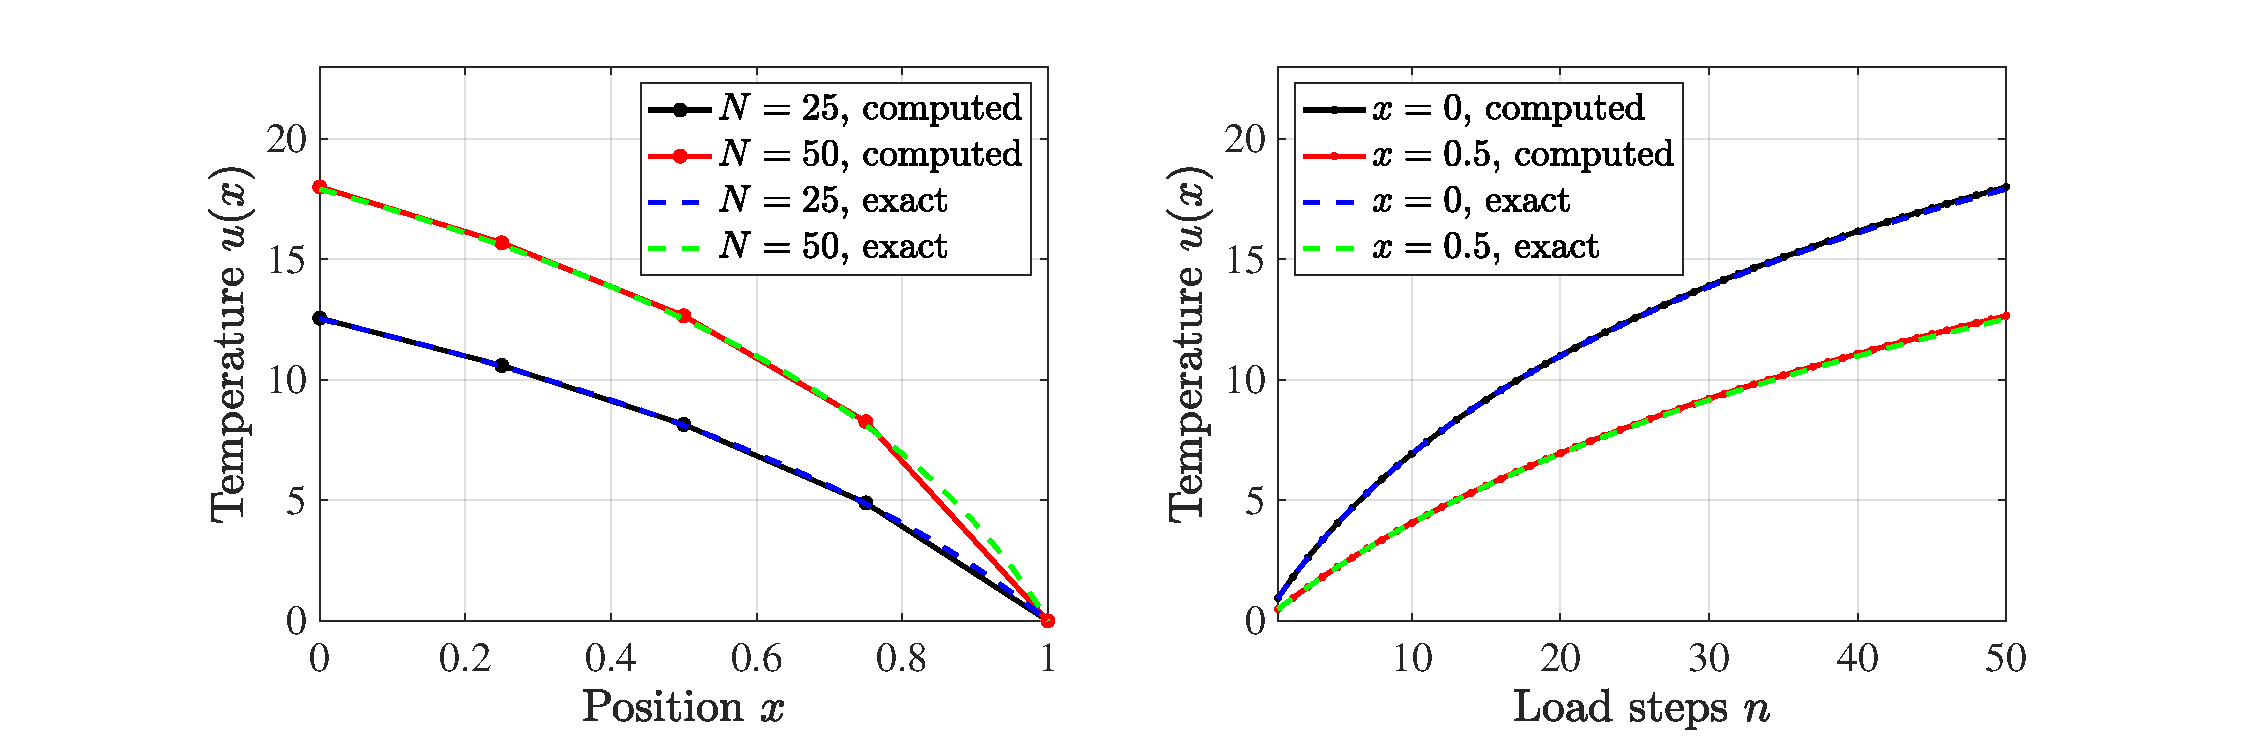
\includegraphics[width=\linewidth]{homework/hw2/hw2_eps_0pt1.pdf}
    \caption{$\epsilon = 0.1$. Left: temperature profile $u(x)$ at load steps 25 and 50. Right: temperature at $x = 0$ and $x = 0.5$ for every load step.}
    \label{fig:hw2_p2_c}
\end{figure}

\begin{figure}[!ht]
    \centering
    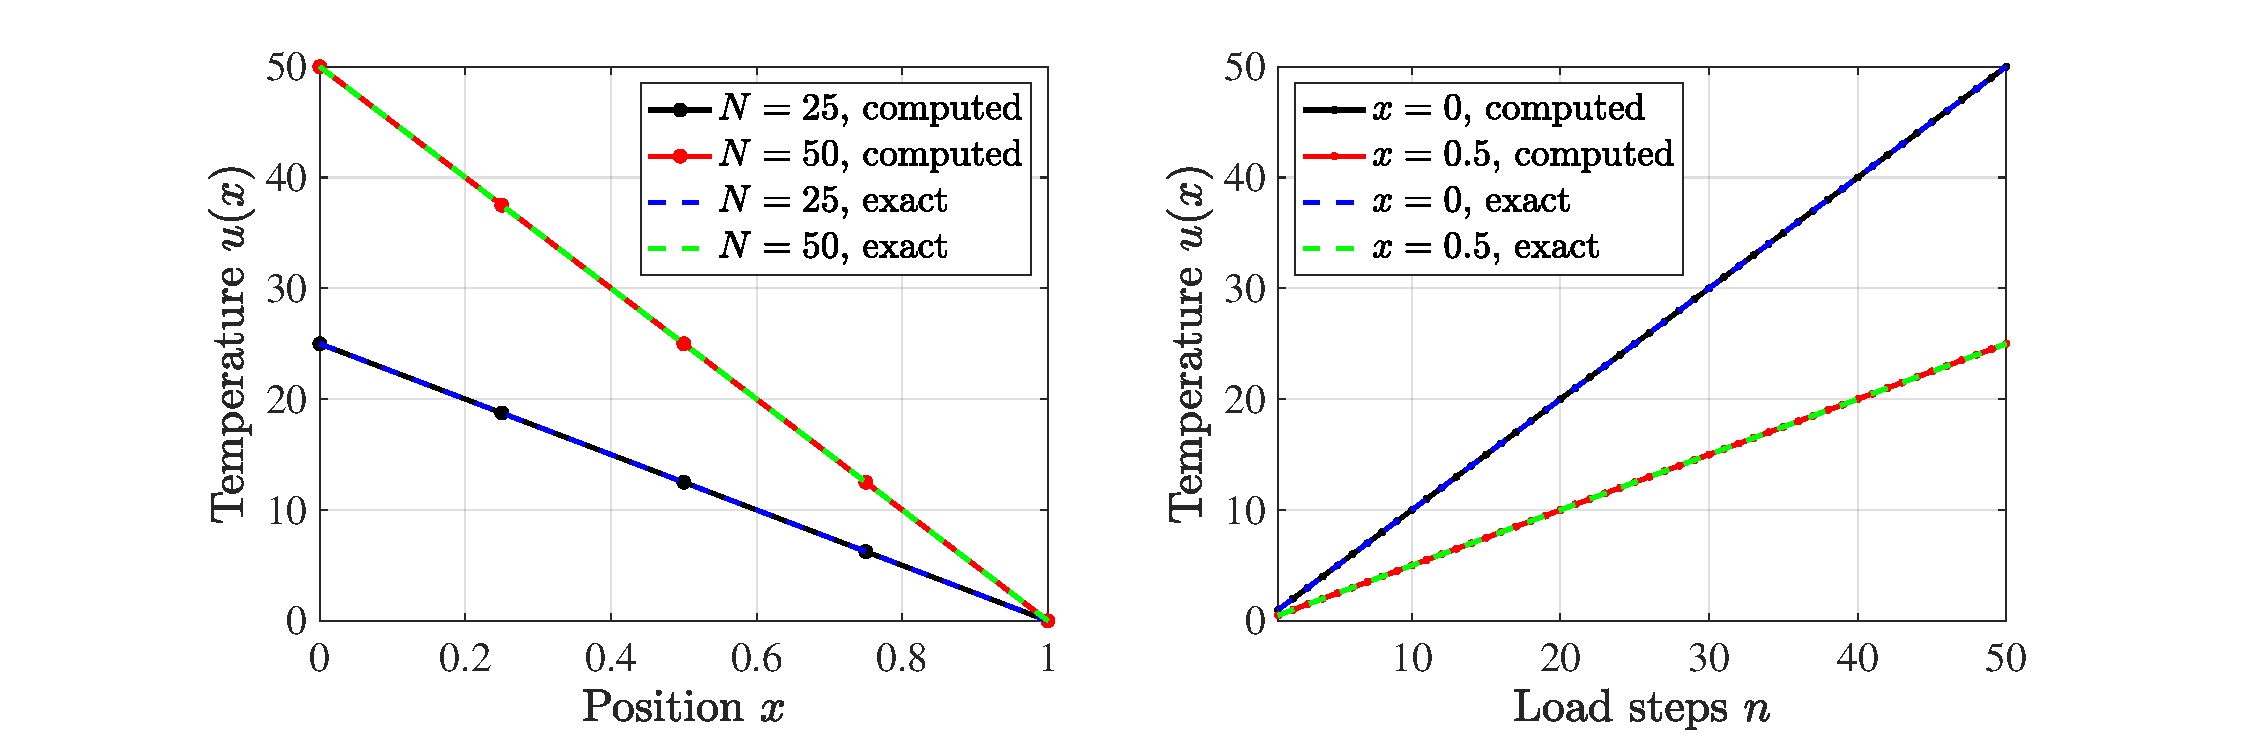
\includegraphics[width=\linewidth]{homework/hw2/hw2_eps_0.pdf}
    \caption{$\epsilon = 0$. Left: temperature profile $u(x)$ at load steps 25 and 50. Right: temperature at $x = 0$ and $x = 0.5$ for every load step.}
    \label{fig:hw2_p2_d}
\end{figure}